% Use the following line _only_ if you're still using LaTeX 2.09.
%\documentstyle[icml2014,epsf,natbib]{article}
% If you rely on Latex2e packages, like most modern people use this:
\documentclass{article}

% use Times
\usepackage{times}
% For figures
\usepackage{graphicx} % more modern
%\usepackage{epsfig} % less modern
\usepackage{subfigure} 

% For citations
\usepackage{natbib}

% For algorithms
\usepackage{algorithm}
\usepackage{algorithmic}

% As of 2011, we use the hyperref package to produce hyperlinks in the
% resulting PDF.  If this breaks your system, please commend out the
% following usepackage line and replace \usepackage{icml2014} with
% \usepackage[nohyperref]{icml2014} above.
\usepackage{hyperref}

% Packages hyperref and algorithmic misbehave sometimes.  We can fix
% this with the following command.
\newcommand{\theHalgorithm}{\arabic{algorithm}}

% Employ the following version of the ``usepackage'' statement for
% submitting the draft version of the paper for review.  This will set
% the note in the first column to ``Under review.  Do not distribute.''
\usepackage{format/icml2014} 
% Employ this version of the ``usepackage'' statement after the paper has
% been accepted, when creating the final version.  This will set the
% note in the first column to ``Proceedings of the...''
%\usepackage[accepted]{icml2014}

\usepackage{times}
\usepackage{hyperref}
\usepackage{url}
\usepackage{color}
\usepackage{preamble}
\definecolor{mydarkblue}{rgb}{0,0.08,0.45}
\hypersetup{ %
    pdftitle={},
    pdfauthor={},
    pdfsubject={},
    pdfkeywords={},
    pdfborder=0 0 0,
    pdfpagemode=UseNone,
    colorlinks=true,
    linkcolor=mydarkblue,
    citecolor=mydarkblue,
    filecolor=mydarkblue,
    urlcolor=mydarkblue,
    pdfview=FitH}
    
    
\usepackage{amsmath, amsfonts, bm, lipsum, capt-of}
\usepackage{natbib, xcolor, wrapfig, booktabs, multirow, caption}
\DeclareCaptionType{copyrightbox}
\usepackage{float}

%\renewcommand{\baselinestretch}{0.99}

\def\ie{i.e.\ }
\def\eg{e.g.\ }
\let\oldemptyset\emptyset
\let\emptyset\varnothing

%\author{
%James Robert Lloyd\\
%University of Cambridge\\
%Department of Engineering\\
%\texttt{jrl44@cam.ac.uk}
%\And
%David Duvenaud\\
%University of Cambridge \\
%Department of Engineering \\
%\texttt{dkd23@cam.ac.uk}
%\And
%Roger Grosse\\
%M.I.T.\\
%Brain and Cognitive Sciences \\
%\texttt{rgrosse@mit.edu}
%\And
%Joshua B. Tenenbaum\\
%M.I.T.\\
%Brain and Cognitive Sciences \\
%\texttt{jbt@mit.edu}
%\And
%Zoubin Ghahramani\\
%University of Cambridge \\
%Department of Engineering \\
%\texttt{zoubin@eng.cam.ac.uk}
%}

\newcommand{\fix}{\marginpar{FIX}}
\newcommand{\new}{\marginpar{NEW}}

\setlength{\marginparwidth}{0.6in}
%%%%%%%%%%%%%%%%%%%%%%%%%%%%%%%%%%%%%%%%%%%%%%%%%%%%%%%%%%
%%%% EDITING HELPER FUNCTIONS  %%%%%%%%%%%%%%%%%%%%%%%%%%%
%%%%%%%%%%%%%%%%%%%%%%%%%%%%%%%%%%%%%%%%%%%%%%%%%%%%%%%%%%

%% NA: needs attention (rough writing whose correctness needs to be verified)
%% TBD: instructions for how to fix a gap ("Describe the propagation by ...")
%% PROBLEM: bug or missing crucial bit 

%% use \fXXX versions of these macros to put additional explanation into a footnote.  
%% The idea is that we don't want to interrupt the flow of the paper or make it 
%% impossible to read because there are a bunch of comments.

%% NA's (and TBDs, those less crucially) should be written so 
%% that they flow with the text.

\definecolor{WowColor}{rgb}{.75,0,.75}
\definecolor{SubtleColor}{rgb}{0,0,.50}

% inline
\newcommand{\NA}[1]{\textcolor{SubtleColor}{ {\tiny \bf ($\star$)} #1}}
\newcommand{\LATER}[1]{\textcolor{SubtleColor}{ {\tiny \bf ($\dagger$)} #1}}
\newcommand{\TBD}[1]{\textcolor{SubtleColor}{ {\tiny \bf (!)} #1}}
\newcommand{\PROBLEM}[1]{\textcolor{WowColor}{ {\bf (!!)} {\bf #1}}}

% as margin notes

\newcounter{margincounter}
\newcommand{\displaycounter}{{\arabic{margincounter}}}
\newcommand{\incdisplaycounter}{{\stepcounter{margincounter}\arabic{margincounter}}}

\newcommand{\fTBD}[1]{\textcolor{SubtleColor}{$\,^{(\incdisplaycounter)}$}\marginpar{\tiny\textcolor{SubtleColor}{ {\tiny $(\displaycounter)$} #1}}}

\newcommand{\fPROBLEM}[1]{\textcolor{WowColor}{$\,^{((\incdisplaycounter))}$}\marginpar{\tiny\textcolor{WowColor}{ {\bf $\mathbf{((\displaycounter))}$} {\bf #1}}}}

\newcommand{\fLATER}[1]{\textcolor{SubtleColor}{$\,^{(\incdisplaycounter\dagger)}$}\marginpar{\tiny\textcolor{SubtleColor}{ {\tiny $(\displaycounter\dagger)$} #1}}}


%% For submission, make all render blank.
%\renewcommand{\LATER}[1]{}
%\renewcommand{\fLATER}[1]{}
%\renewcommand{\TBD}[1]{}
%\renewcommand{\fTBD}[1]{}
%\renewcommand{\PROBLEM}[1]{}
%\renewcommand{\fPROBLEM}[1]{}
%\renewcommand{\NA}[1]{#1}  % Note, NA's pass through!


% The \icmltitle you define below is probably too long as a header.
% Therefore, a short form for the running title is supplied here:
\icmltitlerunning{Kernel posterior predictive checks}

\begin{document} 

\twocolumn[
\icmltitle{Kernel posterior predictive checks}

% It is OKAY to include author information, even for blind
% submissions: the style file will automatically remove it for you
% unless you've provided the [accepted] option to the icml2014
% package.
\icmlauthor{Your Name}{email@yourdomain.edu}
\icmladdress{Your Fantastic Institute,
            314159 Pi St., Palo Alto, CA 94306 USA}
\icmlauthor{Your CoAuthor's Name}{email@coauthordomain.edu}
\icmladdress{Their Fantastic Institute,
            27182 Exp St., Toronto, ON M6H 2T1 CANADA}

% You may provide any keywords that you 
% find helpful for describing your paper; these are used to populate 
% the "keywords" metadata in the PDF but will not be shown in the document
\icmlkeywords{}

\vskip 0.3in
]

\begin{abstract} 
We invetigate the utility of the maximum mean discrepancy two sample test as a means of model checking.
We apply it to several models for unsupervised learning and discover their inaccuracies.
\end{abstract} 

\allowdisplaybreaks

\section{Introduction}

Model checking is an inevitable part of a complete data analysis.
It is going to be especially important as probabilistic programming takes off and people build sophisticated models.

Usually one chooses statistics of interest and evaluates the extent to which the beliefs of the model and realised value on the data align.
But how does one generate these statistics?
Ideally one chooses statistics that are of practical importance.

However, it would also be interesting to find the statistic that most strongly indicates a discrepancy; enter MMD.

Call to arms about a lack of model checking in machine learning literature - find some quotes where new models come from speculations about the form of data.

\section{Background: Model checking}

It can either be interpreted as a Bayesian probability statement.

More usefully it can be related to an estimate of utility of a model for predicting a certain quantity.

However, caution : model checking should not replace model comparison and averaging and posterior predictive $p$-values determine \emph{statistical} significance, not \emph{practical} significance.

\section{Background: Maximum mean discrepancy}

Estimates supremum of difference between mean of functions drawn from some space of functions.
RKHS MMD uses smooth functions to find the discrepancy.
Forms a metric over probability distributions.

\section{Kernel MMD for posterior predictive checking}

Generate lots of data from posterior predictive distribution

\section{Toy examples}

\subsection{Spot the odd one out}

Data generated from mixture of two Gaussians and a uniform ring.
Fit a mixture of Gaussians model.
MMD statistic using default lengthscale heuristic does not show any difference - it is looking for very broad discrepancies.

MMD using smaller lengthscale finds the discrepancy.
Green $\circ$ are data, red $\times$ are locations over-represented by the model, blue $+$ are locations under-represented by the model.

\begin{figure}[ht]
\centering
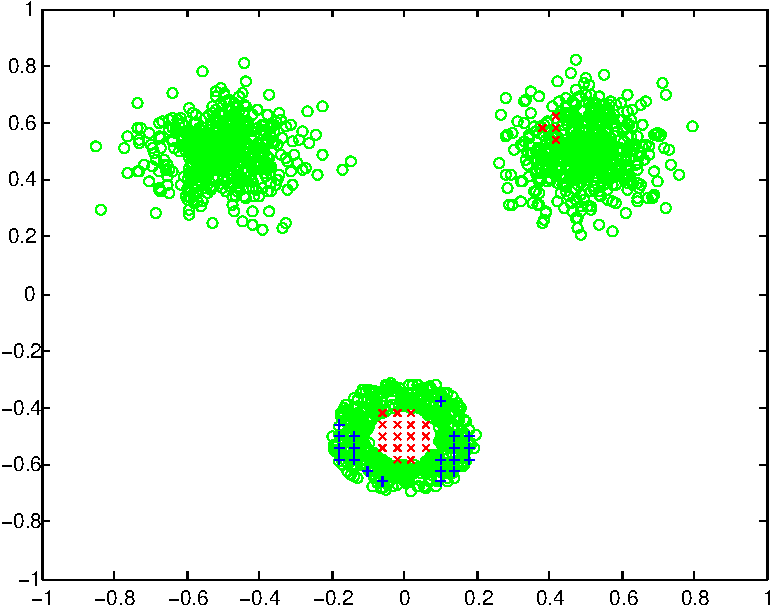
\includegraphics[width=0.98\columnwidth]{figures/blob_blob_ring}
\caption{
An experiment on synthetic data revealing a statistically significant maximum mean discrepancy.
Green $\circ$ are data, red $\times$ are locations over-represented by the model, blue $+$ are locations under-represented by the model.
}
\label{fig:blob_blob_ring}
\end{figure}

MMD has successfully identified the incorrectly modelled cluster.

\section{Case studies}

\subsection{Newcomb speed of light data}

A simple 1-$d$ example.

\subsection{What exactly do neural networks dream about?}

``To recognize shapes, first learn to generate images'' \cite{Hinton2007}.
Restricted Boltzmann Machine (RBM) pretraining of neural networks was shown by \cite{Hinton2006} to learn a deep belief network (DBN) for the training data \ie a generative model.
Subsequently, as well as computing estimates of marginal likelihood and testing errors, it became standard to demonstrate the effectiveness of a neural network by generating samples from the distribution it had learned\fTBD{cite things}.

When trained on the MNIST handwritten digit data, the samples certainly look like digits, but it is hard to detect any systematic anomalies purely by visual inspection.
We now use the kernel two-sample test to investigate how faithfully RBMs and DBNs can capture the distribution over handwritten digits.

\subsubsection{RBMs prefer rounded numbers}

We trained an RBM with architecture $(784)\leftrightarrow(500)\leftrightarrow(10)$ using 15 epochs of PCD-15, a batch size of something and a learning rate of 0.1 (\ie we used the same settings as the code available at (cite deep learning tutorial)).
We generated 3000 independent samples from the learned generative model by initialising the network with a random training image and performing 1000 clamped gibbs updates (without clamping the label pixels, the generative distribution is biased towards certain digits) to generate each image (this is standard \eg \cite{Hinton2007}).

Figure~\ref{fig:rbm_samples} shows the first twenty random samples (\NA{mean activations actually}) from this model.
They certainly look like digits, but has the true distribution over digits been faithfully captured.

\begin{figure}[ht]
\centering
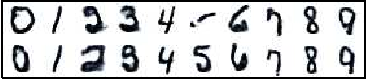
\includegraphics[width=0.98\columnwidth]{figures/rbm_samples}
\caption{
Samples from an RBM (actually the mean activations).
}
\label{fig:rbm_samples}
\end{figure}

Performing a kernel two sample test using the median length scale heuristic resulted in an estimated $p$-value less than 0.001 \ie a clear discrepancy between the model and the data.
We can investigate this discrepancy by examining the images at which the witness function is extremised.
The most over/under represented images are displayed in figure~\ref{fig:rbm_over_under}.
It appears to favour a rounded 2/3/9 whilst it does not like slanty 3, 5 and 8.

\begin{figure}[ht]
\centering
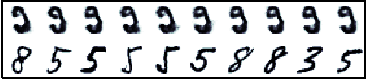
\includegraphics[width=0.98\columnwidth]{figures/rbm_over_under}
\caption{
Over (top row) and under (bottom row) represented images by the RBM.
}
\label{fig:rbm_over_under}
\end{figure}

To test that this was not just a poorly trained single RBM, we trained 1500 RBMs and generated one sample from each and performed the same tests.
The estimated $p$-value was 0.005.
We show the over/under represented images in figure~\ref{fig:many_rbm_over_under}.

\begin{figure}[ht]
\centering
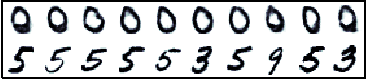
\includegraphics[width=0.98\columnwidth]{figures/many_rbm_over_under}
\caption{
Over (top row) and under (bottom row) represented images by many RBMs.
}
\label{fig:many_rbm_over_under}
\end{figure}

Again we see a fondness for rounded numbers.
This is not digit label bias per se since we were sampling from conditional distributions.
To better probe the round / slanty hypothesis further lets look at conditional distributions.
Figure~\ref{fig:many_rbm_over_under_digit} shows that the RBMs are mislabeling on average - the digits 2 and 5 are close.

\begin{figure}[ht]
\centering
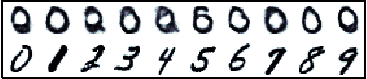
\includegraphics[width=0.98\columnwidth]{figures/many_rbm_over_under_digit}
\caption{
Over (top row) and under (bottom row) represented images by many RBMs - conditional distributions.
}
\label{fig:many_rbm_over_under_digit}
\end{figure}

Now separating by PCA in figure~\ref{fig:many_rbm_over_under}.
It is still mostly curvy against slanty.

\begin{figure}[ht]
\centering
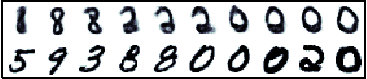
\includegraphics[width=0.98\columnwidth]{figures/many_rbm_over_under_pca}
\caption{
Over (top row) and under (bottom row) represented images by many RBMs - PCA spread.
}
\label{fig:many_rbm_over_under_pca}
\end{figure}

So what is going wrong?
It is probably something to do with round numbers using similar features and therefore these features get better developed faster?

\subsubsection{DBNs also prefer rounded numbers}

\NA{The model below does not use fine tuning - need to do this}

Trained one DBN with architecture $(784)\rightarrow(500)\rightarrow(500)\leftrightarrow(2000)\leftrightarrow(10)$.
Again get a minute $p$-value.
Here are some pictures.

\begin{figure}[ht]
\centering
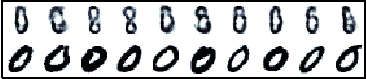
\includegraphics[width=0.98\columnwidth]{figures/dbn_over_under}
\caption{
Over (top row) and under (bottom row) represented images by DBN.
}
\label{fig:many_rbm_over_under}
\end{figure}

\begin{figure}[ht]
\centering
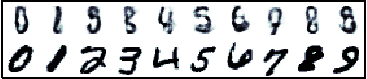
\includegraphics[width=0.98\columnwidth]{figures/dbn_over_under_digit}
\caption{
Over (top row) and under (bottom row) represented images by DBN - conditional distributions.
}
\label{fig:many_rbm_over_under_digit}
\end{figure}

It looks like it is in need of fine tuning - lots of ghosting.

\subsection{Mixture of Gaussians}

\subsection{PCA}

\subsection{GPLVM}

\subsection{Warped mixtures}

\subsection{Alex Matthews latest classification model}

\subsection{GP density model}

\subsection{A generative model for text?}

\section{Discussion}

Do you know what your model is up to right now?
Maybe you should check it is ok.

\bibliography{gpss, library}
\bibliographystyle{format/icml2014}

\end{document} 
